

\chapter{Hesla}

Hesla můžeme vidět všude a ne jen v informatice. 
Pokud se podíváme zpět do historie např. do doby velkého Caesara a jeho šifry, ke které je třeba znát číslo, o které se posouvají znaky ve zprávě. 
Jak tedy můžeme vidět, hesla neslouži pouze k naší autentizaci vůči nějaké službě či serveru. 
Můžeme je také použít k podepsání citlivých dokumentů jako je třeba příloha e-mailu. 
Následně pak nemůžeme popřít jeho poslání. Tomuto se říká elektronický podpis. 

Hesla však mají nejednu nevýhodu. Útočník může s naším, nebo i bez našeho vědění odhalit naše heslo a tím nám narušit naše soukromí. Hesla mohou také být v systémech, které používáme uložena nepatřičným způsobem, jako je například čistý text bez použití žádných ochranných prostředků. 

Hesla též mohou ze systému uniknout. V tomto případě, pokud byla hesla uložena neptřičným způsobem nemusí se potencionální útočník nějak přemáhat, aby uživatele kompromitoval. Proto se zaměříme na to jak mohou a jak skutečně jsou uložena. 

\section{Windows}
% https://cs.wikipedia.org/wiki/NTLM
Windows se chovají jinak v doméně a jinak mimo ní. Pokud je počítač v doméně je preferován autentizační protokol kerberos. V doméně je nastaven jeden nebo více autentikačních serverů přes které se uživatel ověřuje. V současných Windows Server edicích je implementován Kerberos verze 5. Kerberos v základní nastavenim operuje na portu 88 a k šifrování používá symetrickou šifru. 
Pokud počítač není nastaven aby se autentikoval pomocí protokolu Kerberos používají Windows šifrování NTLM. Tento protokol autentizace není oficiálně dokumentován, byl však popsán v projektu Samba. Současná nejnvoější verze je označena NTLMv2.

\subsection{Popis protokolu}

Protokol se řídí sekvencí výzva-odpověď, která vyžaduje, aby mezi klientem a serverem  byly vyměněny celkem tři zprávy (three-way-handshake):

\begin{enumerate}
	\item Klient odešle zprávu obsahující informace o klientem podporovaných nebo požadovaných funkcích (velikosti kryptovacích klíčů, požadavek na vzájemnou autentizaci atd.)
	\item Server odpoví zprávou obsahující podobné informace o serverem podporovaných nebo požadovaných funkcích (čímž klient dokáže vybrat vhodné autentizační parametry) a - nejdůležitější část - náhodnou výzvu (8 bytů, tzv kryptografická sůl).
	\item Klient pak použije výzvu ze zprávy, uživatelské jméno a heslo k vypočtení odpovědi. Volba výpočetní metody je závislá na autentizačních parametrech dohodnutých předešlou zprávou, nicméně obecně lze říci, že aplikuje hašovací funkce MD4 nebo MD5 a šifrování DES.
\end{enumerate}

%https://wiki.wizard32.net/xwiki/bin/view/Penetration%20Testing_Red%20Teaming/NTLM%20Relay%20Attack/
\begin{figure}[!ht]
	\centering
 	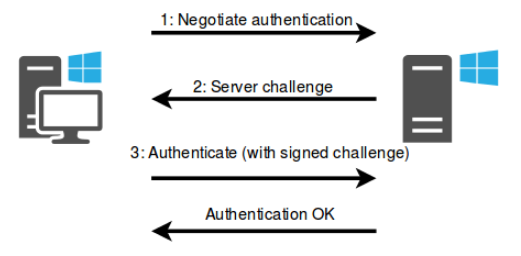
\includegraphics[width=0.8\textwidth, angle=0]{hesla-windows.png}
 	\caption[Hesla windows]{NTLM protokol pro autentizaci.}\label{fig:windows}
\end{figure}

\section{Linux}

Linux jakožto systém, který se skládá pouze ze souborů má též hesla uložena v jednom souboru \path{/etc/shadow}. Hesla v linuxu bývala dříve uložena společně v \path{/etc/passwd}. Kvůli bezpešnosti se však oddělila a v souboru byl otisk nahrazen pismenem x. Hesla jsou uložena pomocí zvolené hašovací funkce. V tabulce níže uvidíme podporované funkce.


% parametry pro table: h! = nejblize
% p{5cm} na zalomovani bunky
\begin{table}[!ht]
  \begin{center}
	\caption{Hašovací funkce}
    \label{tab:Hash funkce}
    \begin{tabular}{|l|l|} 
    	  \hline
      \textbf{ID} & \textbf{Funkce} \\
      \hline

	  1  &  MD5\\
	  2a &  Blowfish\\
	  5  &  SHA-256\\
      6  &  SHA-512\\

      \hline
    \end{tabular}
  \end{center}
\end{table}

%TODO better shadow structure

\section{Hešovací funkce}

% https://link.springer.com/content/pdf/10.1007%2F978-3-540-25937-4_24.pdf
% https://knihy.nic.cz/files/edice/Kryptografie_okolo_nas.pdf

Hešovací funkce je kryptografická funkce, která argumentu o prakticky libovolné délce přiřazuje tzv. heš H, což je číselná hodnota o pevně stanovené délce (typicky o délce 256 až 512 bitů). 
Od hešovací funkce se vyžadují dvě specifické vlastnosti:

\begin{itemize}
	\item \textbf{Jednosměrnost}, což znamená, že určení hodnoty heše je pro zadaný vzor výpočetně snadné, avšak určení hodnoty vzoru ze znalosti jeho heše je prakticky nemožné.
	\item \textbf{Bezkoliznost}, což znamená, že je prakticky nemožné nalézt nějakou dvojici různých vzorů takovou, aby jejich heše byly stejné. V této souvislosti je zapotřebí si uvědomit, že počet číselných posloupností libovolné délky (tj. počet vzorů) je vždy větší než počet posloupností jediné možné délky. Z toho pak plyne, že mnoho vzorů musí mít stejný heš a vznikají tak kolize. Požaduje se však, aby nalezení kolize bylo prakticky nemožné.
\end{itemize}

\begin{figure}[!ht]
	\centering
 	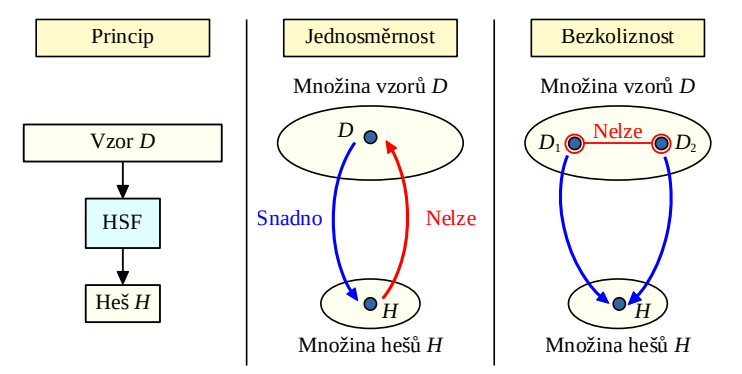
\includegraphics[width=0.8\textwidth, angle=0]{hesla-has.png}
 	\caption[Hesla hešovací funkce]{Hešovací funkce a její vlastnosti.}\label{fig:has}
\end{figure}
 
Kryprografické využití hešovacích funkcí:
 
\begin{itemize}
\item Kontrola integrity (kontrola shodnosti velkých souborů a dat).
\item Automatické dešifrování (souboru, disku apod.).
\item Ukládání a kontrola přihlašovacích hesel. 
\item Prokazování autorství.
\item Jednoznacná identifikace dat (jednoznačná reprezentace vzoru, digitální otisk dat, jednoznacný identifikátor dat, to vše zejména pro digitální podpisy).
\item Prokazování znalosti.
\item Autentizace původu dat.
\item Nepadělatelná kontrola integrity.
\item Pseudonáhodné generátory, derivace klíčů.
\end{itemize}

\subsubsection{MD5}
%http://crypto-world.info/klima/2005/cryptofest_2005.htm#_Toc98987082
%U MD5 tvoří kontext čtyři 32 bitová slova A, B, C a D. Na obrázku vidíme zvětšenu jednu rundu hašování. \( m_i \) je jeden 512 bitový blok zprávy. Ten je rozdělen na 16 32bitových slov \( M_0 M_1 \), \cdots, \( M_{15} \), a tato posloupnost je opakována 4x za sebou (v různých permutacích). 

%Na obrázku vidíme, že v kompresní funkci se kontext "zašifruje" vždy jedním 32bitovým slovem \( M_{i} \). Poznamenejme, že na místě dílčí funkce F v obrázku se po 16 rundách střídají 4 různé (nelineární i lineární) funkce (F, G, H, I) a v každé rundě se využívá jiná konstanta \( K_{i} \). Po 64 rundách dojde ještě k přičtení původního kontextu \( (H_i-1) \) k výsledku podle Davies-Meyerovy konstrukce (xor je nahrazen aritmetickým součtem modulo 232). Tak vznikne nový kontext \( H_{i} \). 

%Pokud by zpráva M měla jen jeden blok, byl by kontext (A, B, C, D) celkovým výsledkem. Pokud ne, pokračuje se stejným způsobem v hašování druhého bloku zprávy m_2 jakoby s inicializační hodnotou \( H_i-1 \). Po zpracování bloku \( m_N \) máme v registrech výslednou 128bitovou haš HN.

\begin{figure}[!ht]
	\centering
 	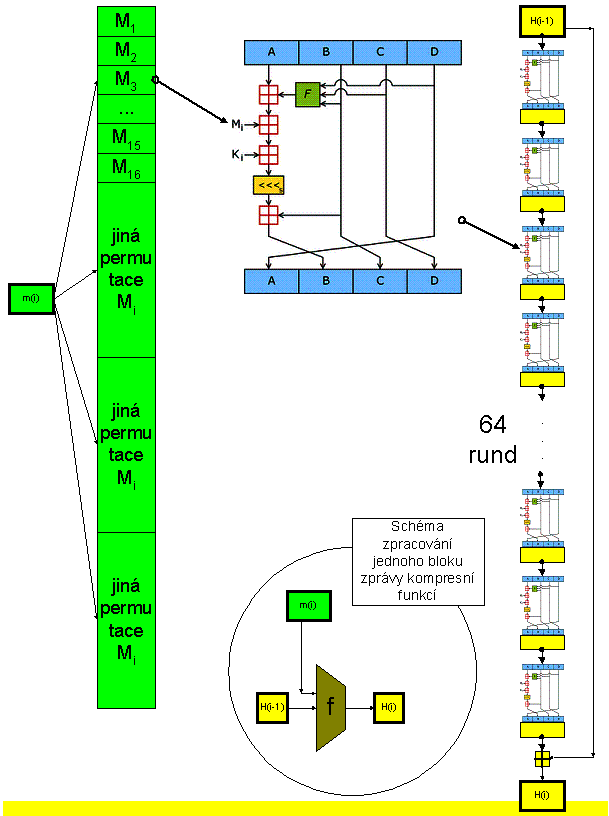
\includegraphics[width=0.8\textwidth, angle=0]{hesla-md5.png}
 	\caption[Hesla a hešovací funkce MD5]{Hešovací funkce MD5.}\label{fig:md5}
\end{figure}

\subsubsection{SHA-1}

Algoritmus SHA (Secure Hash Algorithm) byl zavedený NIST a publikovaný v norme FIPS 180 (1993). Revidovaná verze SHA–1 v normě FIPS–180–1 (1995). SHA–1 umožnuje zpracovat zprávu s %maximální délkou 2^64 − 1 bitů a představuje výstupní hašoví kód s délkou 160b. Vstupní
zpráva M je zpracována po blocích z velkosí 512b. Svým vnitřním fungováním je velice podobná MD5. Liší se zejména v velikosti výstupního řetězce. 

%Blok zprávy Mi
%je zpracováván v 4 × 20 rundách. 160 bitový
%kontext (opet za ˇ cínáme s inicializa ˇ cním vektorem ˇ IV ) je postupneˇ
%"zašifrováván"32b slovem mi pro rundy 0, 1, . . . , 15 a pro rundy
%16, 18, . . . , 79 32b slovem wi

Při inovaci standardu FIPS 180-1 na FIPS 180-2  byly zavedeny 3 nové hašovací algoritmy: SHA-256, SHA-384 a SHA-512. Jejich rozdíly je možné vidět v tabulce. 

%https://www.fit-wiki.cz/_media/%C5%A1kola/p%C5%99edm%C4%9Bty/bez-all.pdf

% parametry pro table: h! = nejblize
% p{5cm} na zalomovani bunky
\begin{table}[!ht]
  \begin{center}
	\caption{SHA-X vlastnosti}
    \label{tab:SHA-X}
    \begin{tabular}{|l|c|c|c|c|} 
    	  \hline
      \textbf{} & \textbf{SHA-1} & \textbf{SHA-256} & \textbf{SHA-384} & \textbf{SHA-512}\\
      \hline
	  Délka haš. kódu 		& 160  & 256  & 384   & 512\\
	  Délka zprávy 			& <264 & <264 & <2128 & <2128\\
	  Velikost bloku 		& 512  & 512  & 1024  & 1024\\
	  Velikost slova 		& 32   & 32   & 64    & 84\\
	  Počet rund 			& 80   & 80   & 80    & 80\\
	  Bezpecnost v bitech 	& 80   & 128  & 192   & 256\\
      \hline
    \end{tabular}
  \end{center}
\end{table}

\section{Útoky na hesla}



\subsection{Hrubou silou}

\subsection{Pomocí masky}

\subsection{Se slovníkem}

\section{Entropie hesla}

\section{Ochrana před různými útoky}


% https://vxempire.xyz/repo/Hash%20Crack.pdf